\PassOptionsToPackage{unicode=true}{hyperref} % options for packages loaded elsewhere
\PassOptionsToPackage{hyphens}{url}
\PassOptionsToPackage{dvipsnames,svgnames*,x11names*}{xcolor}
%
\documentclass[]{article}
\usepackage{lmodern}
\usepackage{amssymb,amsmath}
\usepackage{ifxetex,ifluatex}
\usepackage{fixltx2e} % provides \textsubscript
\ifnum 0\ifxetex 1\fi\ifluatex 1\fi=0 % if pdftex
  \usepackage[T1]{fontenc}
  \usepackage[utf8]{inputenc}
  \usepackage{textcomp} % provides euro and other symbols
\else % if luatex or xelatex
  \usepackage{unicode-math}
  \defaultfontfeatures{Ligatures=TeX,Scale=MatchLowercase}
\fi
% use upquote if available, for straight quotes in verbatim environments
\IfFileExists{upquote.sty}{\usepackage{upquote}}{}
% use microtype if available
\IfFileExists{microtype.sty}{%
\usepackage[]{microtype}
\UseMicrotypeSet[protrusion]{basicmath} % disable protrusion for tt fonts
}{}
\IfFileExists{parskip.sty}{%
\usepackage{parskip}
}{% else
\setlength{\parindent}{0pt}
\setlength{\parskip}{6pt plus 2pt minus 1pt}
}
\usepackage{xcolor}
\usepackage{hyperref}
\hypersetup{
            pdftitle={Module 7: Solutions to recommended Exercises},
            pdfauthor={Emma Skarstein, Michail Spitieris, Stefanie Muff; Department of Mathematical Sciences, NTNU},
            colorlinks=true,
            linkcolor=Maroon,
            filecolor=Maroon,
            citecolor=Blue,
            urlcolor=blue,
            breaklinks=true}
\urlstyle{same}  % don't use monospace font for urls
\usepackage[margin=1in]{geometry}
\usepackage{color}
\usepackage{fancyvrb}
\newcommand{\VerbBar}{|}
\newcommand{\VERB}{\Verb[commandchars=\\\{\}]}
\DefineVerbatimEnvironment{Highlighting}{Verbatim}{commandchars=\\\{\}}
% Add ',fontsize=\small' for more characters per line
\usepackage{framed}
\definecolor{shadecolor}{RGB}{248,248,248}
\newenvironment{Shaded}{\begin{snugshade}}{\end{snugshade}}
\newcommand{\AlertTok}[1]{\textcolor[rgb]{0.94,0.16,0.16}{#1}}
\newcommand{\AnnotationTok}[1]{\textcolor[rgb]{0.56,0.35,0.01}{\textbf{\textit{#1}}}}
\newcommand{\AttributeTok}[1]{\textcolor[rgb]{0.77,0.63,0.00}{#1}}
\newcommand{\BaseNTok}[1]{\textcolor[rgb]{0.00,0.00,0.81}{#1}}
\newcommand{\BuiltInTok}[1]{#1}
\newcommand{\CharTok}[1]{\textcolor[rgb]{0.31,0.60,0.02}{#1}}
\newcommand{\CommentTok}[1]{\textcolor[rgb]{0.56,0.35,0.01}{\textit{#1}}}
\newcommand{\CommentVarTok}[1]{\textcolor[rgb]{0.56,0.35,0.01}{\textbf{\textit{#1}}}}
\newcommand{\ConstantTok}[1]{\textcolor[rgb]{0.00,0.00,0.00}{#1}}
\newcommand{\ControlFlowTok}[1]{\textcolor[rgb]{0.13,0.29,0.53}{\textbf{#1}}}
\newcommand{\DataTypeTok}[1]{\textcolor[rgb]{0.13,0.29,0.53}{#1}}
\newcommand{\DecValTok}[1]{\textcolor[rgb]{0.00,0.00,0.81}{#1}}
\newcommand{\DocumentationTok}[1]{\textcolor[rgb]{0.56,0.35,0.01}{\textbf{\textit{#1}}}}
\newcommand{\ErrorTok}[1]{\textcolor[rgb]{0.64,0.00,0.00}{\textbf{#1}}}
\newcommand{\ExtensionTok}[1]{#1}
\newcommand{\FloatTok}[1]{\textcolor[rgb]{0.00,0.00,0.81}{#1}}
\newcommand{\FunctionTok}[1]{\textcolor[rgb]{0.00,0.00,0.00}{#1}}
\newcommand{\ImportTok}[1]{#1}
\newcommand{\InformationTok}[1]{\textcolor[rgb]{0.56,0.35,0.01}{\textbf{\textit{#1}}}}
\newcommand{\KeywordTok}[1]{\textcolor[rgb]{0.13,0.29,0.53}{\textbf{#1}}}
\newcommand{\NormalTok}[1]{#1}
\newcommand{\OperatorTok}[1]{\textcolor[rgb]{0.81,0.36,0.00}{\textbf{#1}}}
\newcommand{\OtherTok}[1]{\textcolor[rgb]{0.56,0.35,0.01}{#1}}
\newcommand{\PreprocessorTok}[1]{\textcolor[rgb]{0.56,0.35,0.01}{\textit{#1}}}
\newcommand{\RegionMarkerTok}[1]{#1}
\newcommand{\SpecialCharTok}[1]{\textcolor[rgb]{0.00,0.00,0.00}{#1}}
\newcommand{\SpecialStringTok}[1]{\textcolor[rgb]{0.31,0.60,0.02}{#1}}
\newcommand{\StringTok}[1]{\textcolor[rgb]{0.31,0.60,0.02}{#1}}
\newcommand{\VariableTok}[1]{\textcolor[rgb]{0.00,0.00,0.00}{#1}}
\newcommand{\VerbatimStringTok}[1]{\textcolor[rgb]{0.31,0.60,0.02}{#1}}
\newcommand{\WarningTok}[1]{\textcolor[rgb]{0.56,0.35,0.01}{\textbf{\textit{#1}}}}
\usepackage{graphicx,grffile}
\makeatletter
\def\maxwidth{\ifdim\Gin@nat@width>\linewidth\linewidth\else\Gin@nat@width\fi}
\def\maxheight{\ifdim\Gin@nat@height>\textheight\textheight\else\Gin@nat@height\fi}
\makeatother
% Scale images if necessary, so that they will not overflow the page
% margins by default, and it is still possible to overwrite the defaults
% using explicit options in \includegraphics[width, height, ...]{}
\setkeys{Gin}{width=\maxwidth,height=\maxheight,keepaspectratio}
\setlength{\emergencystretch}{3em}  % prevent overfull lines
\providecommand{\tightlist}{%
  \setlength{\itemsep}{0pt}\setlength{\parskip}{0pt}}
\setcounter{secnumdepth}{0}
% Redefines (sub)paragraphs to behave more like sections
\ifx\paragraph\undefined\else
\let\oldparagraph\paragraph
\renewcommand{\paragraph}[1]{\oldparagraph{#1}\mbox{}}
\fi
\ifx\subparagraph\undefined\else
\let\oldsubparagraph\subparagraph
\renewcommand{\subparagraph}[1]{\oldsubparagraph{#1}\mbox{}}
\fi

% set default figure placement to htbp
\makeatletter
\def\fps@figure{htbp}
\makeatother

\usepackage{etoolbox}
\makeatletter
\providecommand{\subtitle}[1]{% add subtitle to \maketitle
  \apptocmd{\@title}{\par {\large #1 \par}}{}{}
}
\makeatother

\title{Module 7: Solutions to recommended Exercises}
\providecommand{\subtitle}[1]{}
\subtitle{TMA4268 Statistical Learning V2021}
\author{Emma Skarstein, Michail Spitieris, Stefanie Muff \and Department of Mathematical Sciences, NTNU}
\date{March 2, 2021}

\begin{document}
\maketitle

\hypertarget{problem-1}{%
\subsection{Problem 1}\label{problem-1}}

The code below performs polynomial regression of degree 1, 2, 3 and 4.
The function \texttt{sapply()} is an efficient for-loop. We iterate over
all degrees to plot the fitted values and compute the test error.
Finally we plot the test error for each polynomial degree.

\begin{Shaded}
\begin{Highlighting}[]
\KeywordTok{library}\NormalTok{(ISLR)}
\CommentTok{# extract only the two variables from Auto}
\NormalTok{ds =}\StringTok{ }\NormalTok{Auto[}\KeywordTok{c}\NormalTok{(}\StringTok{"horsepower"}\NormalTok{, }\StringTok{"mpg"}\NormalTok{)]}
\NormalTok{n =}\StringTok{ }\KeywordTok{nrow}\NormalTok{(ds)}
\CommentTok{# which degrees we will look at}
\NormalTok{deg =}\StringTok{ }\DecValTok{1}\OperatorTok{:}\DecValTok{4}
\KeywordTok{set.seed}\NormalTok{(}\DecValTok{1}\NormalTok{)}
\CommentTok{# training ids for training set}
\NormalTok{tr =}\StringTok{ }\KeywordTok{sample.int}\NormalTok{(n, n}\OperatorTok{/}\DecValTok{2}\NormalTok{)}
\CommentTok{# plot of training data}
\KeywordTok{plot}\NormalTok{(ds[tr, ], }\DataTypeTok{col =} \StringTok{"darkgrey"}\NormalTok{, }\DataTypeTok{main =} \StringTok{"Polynomial regression"}\NormalTok{)}

\CommentTok{# which colors we will plot the lines with}
\NormalTok{co =}\StringTok{ }\KeywordTok{rainbow}\NormalTok{(}\KeywordTok{length}\NormalTok{(deg))}
\CommentTok{# iterate over all degrees (1:4) - could also use a for-loop here}
\NormalTok{MSE =}\StringTok{ }\KeywordTok{sapply}\NormalTok{(deg, }\ControlFlowTok{function}\NormalTok{(d) \{}
    \CommentTok{# fit model with this degree}
\NormalTok{    mod =}\StringTok{ }\KeywordTok{lm}\NormalTok{(mpg }\OperatorTok{~}\StringTok{ }\KeywordTok{poly}\NormalTok{(horsepower, d), ds[tr, ])}
    \CommentTok{# add lines to the plot - use fitted values (for mpg) and horsepower from}
    \CommentTok{# training set}
    \KeywordTok{lines}\NormalTok{(}\KeywordTok{cbind}\NormalTok{(ds[tr, }\DecValTok{1}\NormalTok{], mod}\OperatorTok{$}\NormalTok{fit)[}\KeywordTok{order}\NormalTok{(ds[tr, }\DecValTok{1}\NormalTok{]), ], }\DataTypeTok{col =}\NormalTok{ co[d])}
    \CommentTok{# calculate mean MSE - this is returned in the MSE variable}
    \KeywordTok{mean}\NormalTok{((}\KeywordTok{predict}\NormalTok{(mod, ds[}\OperatorTok{-}\NormalTok{tr, ]) }\OperatorTok{-}\StringTok{ }\NormalTok{ds[}\OperatorTok{-}\NormalTok{tr, }\DecValTok{2}\NormalTok{])}\OperatorTok{^}\DecValTok{2}\NormalTok{)}
\NormalTok{\})}
\CommentTok{# add legend to see which color corresponds to which line}
\KeywordTok{legend}\NormalTok{(}\StringTok{"topright"}\NormalTok{, }\DataTypeTok{legend =} \KeywordTok{paste}\NormalTok{(}\StringTok{"d ="}\NormalTok{, deg), }\DataTypeTok{lty =} \DecValTok{1}\NormalTok{, }\DataTypeTok{col =}\NormalTok{ co)}
\end{Highlighting}
\end{Shaded}

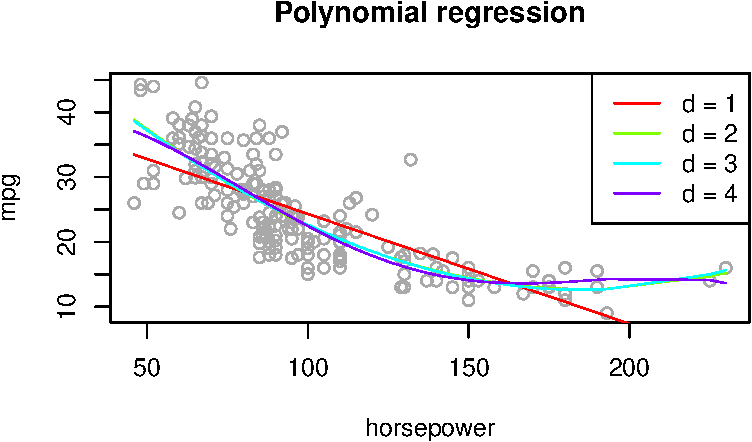
\includegraphics{RecEx7-sol_files/figure-latex/unnamed-chunk-1-1.pdf}

\begin{Shaded}
\begin{Highlighting}[]
\CommentTok{# plot MSE}
\KeywordTok{plot}\NormalTok{(MSE, }\DataTypeTok{type =} \StringTok{"o"}\NormalTok{, }\DataTypeTok{pch =} \DecValTok{16}\NormalTok{, }\DataTypeTok{xlab =} \StringTok{"degree"}\NormalTok{, }\DataTypeTok{main =} \StringTok{"Test error"}\NormalTok{)}
\end{Highlighting}
\end{Shaded}

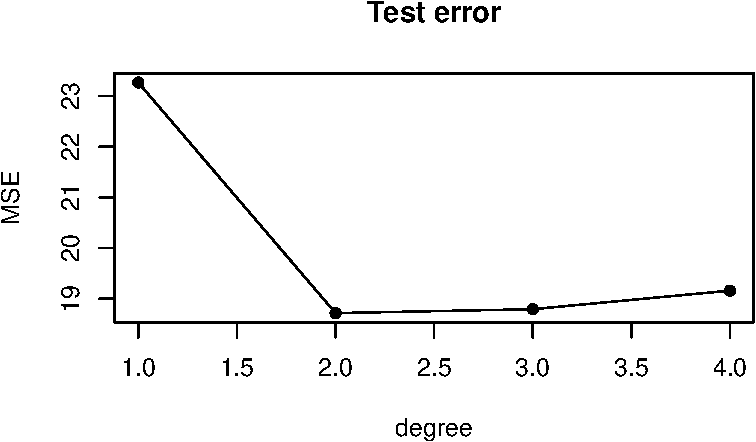
\includegraphics{RecEx7-sol_files/figure-latex/unnamed-chunk-1-2.pdf}

The same solution using \texttt{ggplot} is shown below.

\begin{Shaded}
\begin{Highlighting}[]
\CommentTok{# solution with ggplot}
\KeywordTok{library}\NormalTok{(ISLR)}
\KeywordTok{library}\NormalTok{(ggplot2)}
\CommentTok{# extract only the two variables from Auto}
\NormalTok{ds =}\StringTok{ }\NormalTok{Auto[}\KeywordTok{c}\NormalTok{(}\StringTok{"horsepower"}\NormalTok{, }\StringTok{"mpg"}\NormalTok{)]}
\NormalTok{n =}\StringTok{ }\KeywordTok{nrow}\NormalTok{(ds)}
\CommentTok{# which degrees we will look at}
\NormalTok{deg =}\StringTok{ }\DecValTok{1}\OperatorTok{:}\DecValTok{4}
\KeywordTok{set.seed}\NormalTok{(}\DecValTok{1}\NormalTok{)}
\CommentTok{# training ids for training set}
\NormalTok{tr =}\StringTok{ }\KeywordTok{sample.int}\NormalTok{(n, n}\OperatorTok{/}\DecValTok{2}\NormalTok{)}
\CommentTok{# plot of training data}
\KeywordTok{ggplot}\NormalTok{(}\DataTypeTok{data =}\NormalTok{ ds[tr, ], }\KeywordTok{aes}\NormalTok{(}\DataTypeTok{x =}\NormalTok{ horsepower, }\DataTypeTok{y =}\NormalTok{ mpg)) }\OperatorTok{+}\StringTok{ }\KeywordTok{geom_point}\NormalTok{(}\DataTypeTok{color =} \StringTok{"darkgrey"}\NormalTok{) }\OperatorTok{+}\StringTok{ }
\StringTok{    }\KeywordTok{labs}\NormalTok{(}\DataTypeTok{title =} \StringTok{"Polynomial regression"}\NormalTok{)}
\end{Highlighting}
\end{Shaded}

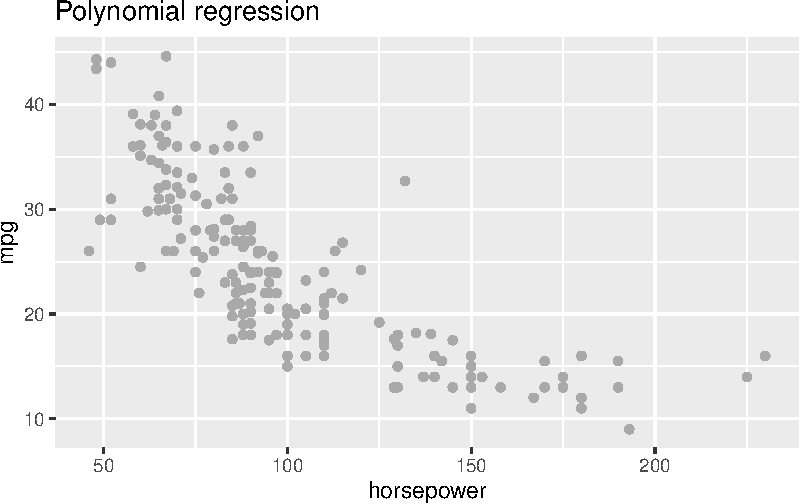
\includegraphics{RecEx7-sol_files/figure-latex/unnamed-chunk-2-1.pdf}

\begin{Shaded}
\begin{Highlighting}[]
\CommentTok{# iterate over all degrees (1:4) - could also use a for-loop here}
\NormalTok{dat =}\StringTok{ }\KeywordTok{c}\NormalTok{()  }\CommentTok{#make a empty variable to store predicted values}
\ControlFlowTok{for}\NormalTok{ (d }\ControlFlowTok{in}\NormalTok{ deg) \{}
    \CommentTok{# fit model with this degree}
\NormalTok{    mod =}\StringTok{ }\KeywordTok{lm}\NormalTok{(mpg }\OperatorTok{~}\StringTok{ }\KeywordTok{poly}\NormalTok{(horsepower, d), ds[tr, ])}
    \CommentTok{# dataframe of predicted values - use fitted values (for mpg) and horsepower}
    \CommentTok{# from training set and add column (factor) for degree}
\NormalTok{    dat =}\StringTok{ }\KeywordTok{rbind}\NormalTok{(dat, }\KeywordTok{data.frame}\NormalTok{(}\DataTypeTok{horsepower =}\NormalTok{ ds[tr, }\DecValTok{1}\NormalTok{], }\DataTypeTok{mpg =}\NormalTok{ mod}\OperatorTok{$}\NormalTok{fit, }\DataTypeTok{degree =} \KeywordTok{as.factor}\NormalTok{(}\KeywordTok{rep}\NormalTok{(d, }
        \KeywordTok{length}\NormalTok{(mod}\OperatorTok{$}\NormalTok{fit)))))}
    \CommentTok{# calculate mean MSE - this is returned in the MSE variable}
\NormalTok{    MSE[d] =}\StringTok{ }\KeywordTok{mean}\NormalTok{((}\KeywordTok{predict}\NormalTok{(mod, ds[}\OperatorTok{-}\NormalTok{tr, ]) }\OperatorTok{-}\StringTok{ }\NormalTok{ds[}\OperatorTok{-}\NormalTok{tr, }\DecValTok{2}\NormalTok{])}\OperatorTok{^}\DecValTok{2}\NormalTok{)}
\NormalTok{\}}
\CommentTok{# plot fitted values for different degrees}
\KeywordTok{ggplot}\NormalTok{(}\DataTypeTok{data =}\NormalTok{ ds[tr, ], }\KeywordTok{aes}\NormalTok{(}\DataTypeTok{x =}\NormalTok{ horsepower, }\DataTypeTok{y =}\NormalTok{ mpg)) }\OperatorTok{+}\StringTok{ }\KeywordTok{geom_point}\NormalTok{(}\DataTypeTok{color =} \StringTok{"darkgrey"}\NormalTok{) }\OperatorTok{+}\StringTok{ }
\StringTok{    }\KeywordTok{labs}\NormalTok{(}\DataTypeTok{title =} \StringTok{"Polynomial regression"}\NormalTok{) }\OperatorTok{+}\StringTok{ }\KeywordTok{geom_line}\NormalTok{(}\DataTypeTok{data =}\NormalTok{ dat, }\KeywordTok{aes}\NormalTok{(}\DataTypeTok{x =}\NormalTok{ horsepower, }
    \DataTypeTok{y =}\NormalTok{ mpg, }\DataTypeTok{color =}\NormalTok{ degree))}
\end{Highlighting}
\end{Shaded}

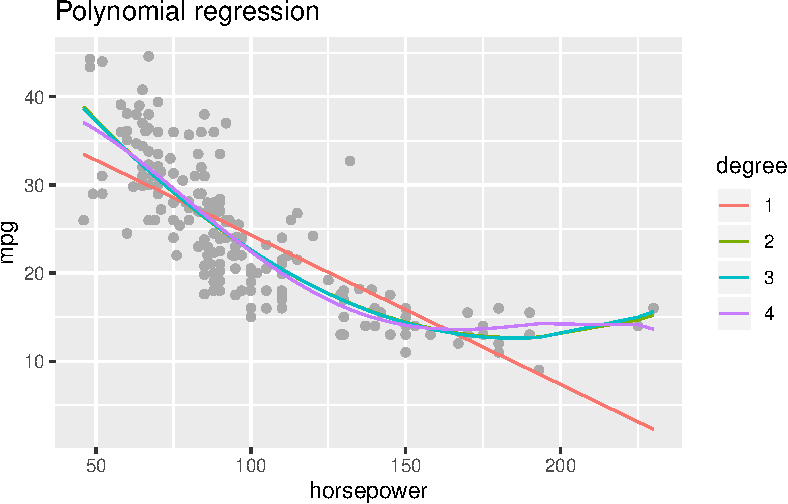
\includegraphics{RecEx7-sol_files/figure-latex/unnamed-chunk-2-2.pdf}

\begin{Shaded}
\begin{Highlighting}[]
\CommentTok{# plot MSE}
\NormalTok{MSEdata =}\StringTok{ }\KeywordTok{data.frame}\NormalTok{(}\DataTypeTok{MSE =}\NormalTok{ MSE, }\DataTypeTok{degree =} \DecValTok{1}\OperatorTok{:}\DecValTok{4}\NormalTok{)}
\KeywordTok{ggplot}\NormalTok{(}\DataTypeTok{data =}\NormalTok{ MSEdata, }\KeywordTok{aes}\NormalTok{(}\DataTypeTok{x =}\NormalTok{ degree, }\DataTypeTok{y =}\NormalTok{ MSE)) }\OperatorTok{+}\StringTok{ }\KeywordTok{geom_line}\NormalTok{() }\OperatorTok{+}\StringTok{ }\KeywordTok{geom_point}\NormalTok{() }\OperatorTok{+}\StringTok{ }
\StringTok{    }\KeywordTok{labs}\NormalTok{(}\DataTypeTok{title =} \StringTok{"Test error"}\NormalTok{)}
\end{Highlighting}
\end{Shaded}

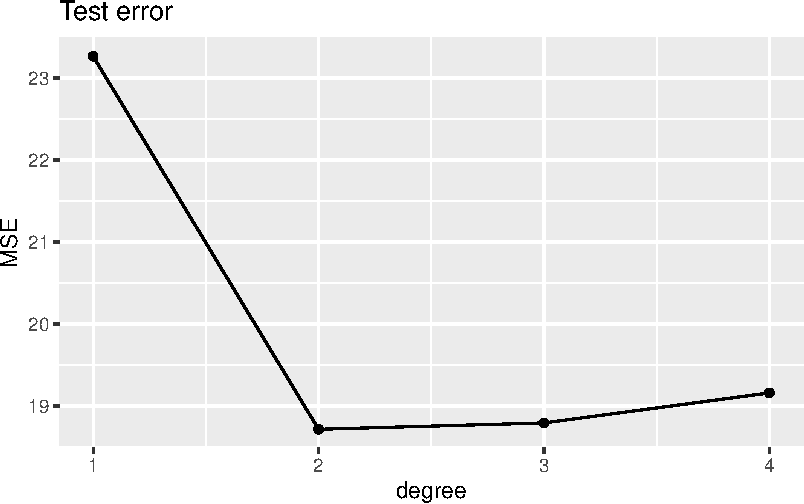
\includegraphics{RecEx7-sol_files/figure-latex/unnamed-chunk-2-3.pdf}

\hypertarget{problem-2}{%
\subsection{Problem 2}\label{problem-2}}

We use \texttt{factor(origin)} for conversion to a factor variable. The
function \texttt{predict(...,\ se\ =\ T)} gives fitted values with
standard errors.

\begin{Shaded}
\begin{Highlighting}[]
\KeywordTok{attach}\NormalTok{(Auto)}
\CommentTok{# fit model}
\NormalTok{fit =}\StringTok{ }\KeywordTok{lm}\NormalTok{(mpg }\OperatorTok{~}\StringTok{ }\KeywordTok{factor}\NormalTok{(origin))}
\CommentTok{# make a new dataset of the origins to predict the mpg for the different}
\CommentTok{# origins}
\NormalTok{new =}\StringTok{ }\KeywordTok{data.frame}\NormalTok{(}\DataTypeTok{origin =} \KeywordTok{as.factor}\NormalTok{(}\KeywordTok{sort}\NormalTok{(}\KeywordTok{unique}\NormalTok{(origin))))}
\CommentTok{# predicted values and standard errors}
\NormalTok{pred =}\StringTok{ }\KeywordTok{predict}\NormalTok{(fit, new, }\DataTypeTok{se =}\NormalTok{ T)}
\CommentTok{# dataframe including CI (z_alpha/2 = 1.96)}
\NormalTok{dat =}\StringTok{ }\KeywordTok{data.frame}\NormalTok{(}\DataTypeTok{origin =}\NormalTok{ new, }\DataTypeTok{mpg =}\NormalTok{ pred}\OperatorTok{$}\NormalTok{fit, }\DataTypeTok{lwr =}\NormalTok{ pred}\OperatorTok{$}\NormalTok{fit }\OperatorTok{-}\StringTok{ }\FloatTok{1.96} \OperatorTok{*}\StringTok{ }\NormalTok{pred}\OperatorTok{$}\NormalTok{se.fit, }
    \DataTypeTok{upr =}\NormalTok{ pred}\OperatorTok{$}\NormalTok{fit }\OperatorTok{+}\StringTok{ }\FloatTok{1.96} \OperatorTok{*}\StringTok{ }\NormalTok{pred}\OperatorTok{$}\NormalTok{se.fit)}
\CommentTok{# plot the fitted/predicted values and CI}
\KeywordTok{ggplot}\NormalTok{(dat, }\KeywordTok{aes}\NormalTok{(}\DataTypeTok{x =}\NormalTok{ origin, }\DataTypeTok{y =}\NormalTok{ mpg)) }\OperatorTok{+}\StringTok{ }\KeywordTok{geom_point}\NormalTok{() }\OperatorTok{+}\StringTok{ }\KeywordTok{geom_segment}\NormalTok{(}\KeywordTok{aes}\NormalTok{(}\DataTypeTok{x =}\NormalTok{ origin, }
    \DataTypeTok{y =}\NormalTok{ lwr, }\DataTypeTok{xend =}\NormalTok{ origin, }\DataTypeTok{yend =}\NormalTok{ upr)) }\OperatorTok{+}\StringTok{ }\KeywordTok{scale_x_discrete}\NormalTok{(}\DataTypeTok{labels =} \KeywordTok{c}\NormalTok{(}\StringTok{`}\DataTypeTok{1}\StringTok{`}\NormalTok{ =}\StringTok{ "1.American"}\NormalTok{, }
    \StringTok{`}\DataTypeTok{2}\StringTok{`}\NormalTok{ =}\StringTok{ "2.European"}\NormalTok{, }\StringTok{`}\DataTypeTok{3}\StringTok{`}\NormalTok{ =}\StringTok{ "3.Japanese"}\NormalTok{))}
\end{Highlighting}
\end{Shaded}

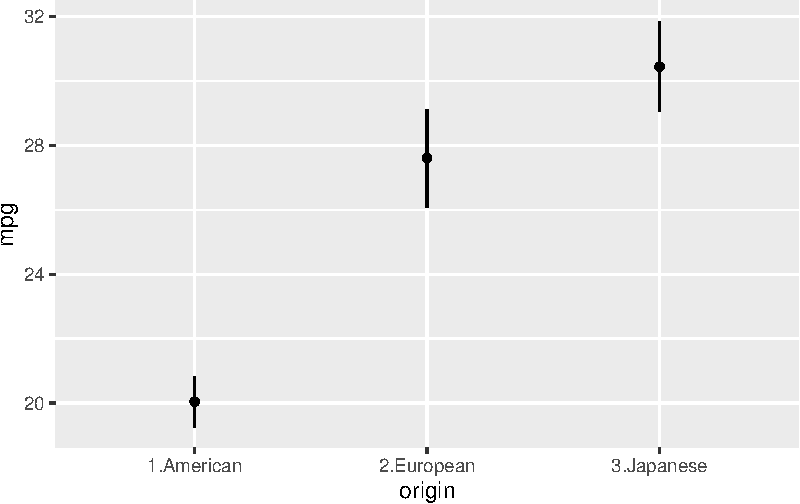
\includegraphics{RecEx7-sol_files/figure-latex/unnamed-chunk-3-1.pdf}

\hypertarget{problem-3}{%
\subsection{Problem 3}\label{problem-3}}

The request is a design matrix for a natural spline with \(X =\)
\texttt{year} and one knot \(c_1 = 2006\). The boundary knots be the
extreme values of \texttt{year}, that is \(c_0 = 2003\) and
\(c_2 = 2009\). A general basis for a natural spline is

\[
b_1(x_i) = x_i, \quad b_{k+2}(x_i) = d_k(x_i)-d_K(x_i),\; k = 0, \ldots, K - 1,\\
\] \[
d_k(x_i) = \frac{(x_i-c_k)^3_+-(x_i-c_{K+1})^3_+}{c_{K+1}-c_k}.
\] In our case we have one internal knot, that is \(K=1\). Thus, \(k\)
takes only the value 0. The two basis functions are

\begin{align*}
b_1(x_i) &= x_i,\\
b_2(x_i) &= d_0(x_i)-d_1(x_i)\\
&= \frac{(x_i-c_0)^3_+-(x_i-c_2)^3_+}{c_2-c_0} - \frac{(x_i-c_1)^3_+-(x_i-c_2)^3_+}{c_2-c_1}\\
&= \frac{1}{c_2-c_0}(x_i-c_0)^3_+ - \frac{1}{c_2-c_1}(x_i-c_1)^3_+ + \left(\frac{1}{c_2-c_1}-\frac{1}{c_2-c_0}\right)(x_i-c_{2})^3_+\\
&= \frac{1}{6}(x_i-2003)^3_+ - \frac{1}{3}(x_i-2006)^3_+ + \frac{1}{6}(x_i-2009)^3_+.
\end{align*}

The design matrix is obtained by \(\{\mathbf X_2\}_{ij} = b_j(x_i)\). We
can simplify the second basis function more by using the fact that the
boundary knots are the extreme values of \(x_i\), that is
\(2003 \leq x_i \leq 2009\), and thus \(\frac{1}{6}(x_i-2009)^3_+=0\).
Thus, \[
b_2(x_i) = \frac{1}{6}(x_i-2003)^3 - \frac{1}{3}(x_i-2006)^3_+.
\]

\hypertarget{problem-4}{%
\subsection{Problem 4}\label{problem-4}}

The matrix \(\mathbf X\) is obtained by using \texttt{cbind()} to join
an intercept, a cubic spline, a natural cubic spline and a factor.

\begin{Shaded}
\begin{Highlighting}[]
\KeywordTok{library}\NormalTok{(ISLR)}
\KeywordTok{attach}\NormalTok{(Wage)}
\CommentTok{# install.packages('gam')}
\KeywordTok{library}\NormalTok{(gam)}

\CommentTok{# Write a couple of functions first, which will be used to produce the}
\CommentTok{# components of the design matrix We write separate functions to generate}
\CommentTok{# X_1, X_2 and X_3 (the three components of the model) X_1: The function}
\CommentTok{# mybs() generates basis functions for the cubic spline}
\NormalTok{mybs =}\StringTok{ }\ControlFlowTok{function}\NormalTok{(x, knots) }\KeywordTok{cbind}\NormalTok{(x, x}\OperatorTok{^}\DecValTok{2}\NormalTok{, x}\OperatorTok{^}\DecValTok{3}\NormalTok{, }\KeywordTok{sapply}\NormalTok{(knots, }\ControlFlowTok{function}\NormalTok{(y) }\KeywordTok{pmax}\NormalTok{(}\DecValTok{0}\NormalTok{, }
\NormalTok{    x }\OperatorTok{-}\StringTok{ }\NormalTok{y)}\OperatorTok{^}\DecValTok{3}\NormalTok{))}

\CommentTok{# X_2: The function myns() generates basis functions for the natural cubic}
\CommentTok{# spline; d() is a helper function}
\NormalTok{d =}\StringTok{ }\ControlFlowTok{function}\NormalTok{(c, cK, x) (}\KeywordTok{pmax}\NormalTok{(}\DecValTok{0}\NormalTok{, x }\OperatorTok{-}\StringTok{ }\NormalTok{c)}\OperatorTok{^}\DecValTok{3} \OperatorTok{-}\StringTok{ }\KeywordTok{pmax}\NormalTok{(}\DecValTok{0}\NormalTok{, x }\OperatorTok{-}\StringTok{ }\NormalTok{cK)}\OperatorTok{^}\DecValTok{3}\NormalTok{)}\OperatorTok{/}\NormalTok{(cK }\OperatorTok{-}\StringTok{ }\NormalTok{c)}
\NormalTok{myns =}\StringTok{ }\ControlFlowTok{function}\NormalTok{(x, knots) \{}
\NormalTok{    kn =}\StringTok{ }\KeywordTok{c}\NormalTok{(}\KeywordTok{min}\NormalTok{(x), knots, }\KeywordTok{max}\NormalTok{(x))}
\NormalTok{    K =}\StringTok{ }\KeywordTok{length}\NormalTok{(kn)}
\NormalTok{    sub =}\StringTok{ }\KeywordTok{d}\NormalTok{(kn[K }\OperatorTok{-}\StringTok{ }\DecValTok{1}\NormalTok{], kn[K], x)}
    \KeywordTok{cbind}\NormalTok{(x, }\KeywordTok{sapply}\NormalTok{(kn[}\DecValTok{1}\OperatorTok{:}\NormalTok{(K }\OperatorTok{-}\StringTok{ }\DecValTok{2}\NormalTok{)], d, kn[K], x) }\OperatorTok{-}\StringTok{ }\NormalTok{sub)}
\NormalTok{\}}

\CommentTok{# X_3: The function myfactor() generates the dummy-basis functions for a}
\CommentTok{# factor covariate, building on the R-function model.matrix()}
\NormalTok{myfactor =}\StringTok{ }\ControlFlowTok{function}\NormalTok{(x) }\KeywordTok{model.matrix}\NormalTok{(}\OperatorTok{~}\NormalTok{x)[, }\DecValTok{-1}\NormalTok{]}

\CommentTok{# Once these functions are prepared, we can generate the model matrix X =}
\CommentTok{# (1,X_1, X_2, X_3) as a one-liner}
\NormalTok{X =}\StringTok{ }\KeywordTok{cbind}\NormalTok{(}\DecValTok{1}\NormalTok{, }\KeywordTok{mybs}\NormalTok{(age, }\KeywordTok{c}\NormalTok{(}\DecValTok{40}\NormalTok{, }\DecValTok{60}\NormalTok{)), }\KeywordTok{myns}\NormalTok{(year, }\DecValTok{2006}\NormalTok{), }\KeywordTok{myfactor}\NormalTok{(education))}
\end{Highlighting}
\end{Shaded}

We have now created a model matrix \(\mathbf X\) ``by hand''. The thing
we wanted to illustrate with this exercise is that this hand-made matrix
does not correspond to the internal representation of the model matrix
that we would direclty get using the \texttt{gam()} function:

\begin{Shaded}
\begin{Highlighting}[]
\NormalTok{X_gam <-}\StringTok{ }\KeywordTok{model.matrix}\NormalTok{(}\OperatorTok{~}\KeywordTok{bs}\NormalTok{(age, }\DataTypeTok{knots =} \KeywordTok{c}\NormalTok{(}\DecValTok{40}\NormalTok{, }\DecValTok{60}\NormalTok{)) }\OperatorTok{+}\StringTok{ }\KeywordTok{ns}\NormalTok{(year, }\DataTypeTok{knots =} \DecValTok{2006}\NormalTok{) }\OperatorTok{+}\StringTok{ }
\StringTok{    }\NormalTok{education)}
\end{Highlighting}
\end{Shaded}

\begin{Shaded}
\begin{Highlighting}[]
\CommentTok{# Anyway, if we now use our model matrix to fit a linear regression model}
\CommentTok{# (excluding the intercept -1, because the first column of X already}
\CommentTok{# contains only 1's and thus encodes for an intercept), we can obtain}
\CommentTok{# predicted values for yhat}
\NormalTok{myhat =}\StringTok{ }\KeywordTok{lm}\NormalTok{(wage }\OperatorTok{~}\StringTok{ }\NormalTok{X }\OperatorTok{-}\StringTok{ }\DecValTok{1}\NormalTok{)}\OperatorTok{$}\NormalTok{fit}

\CommentTok{# Comparing to the fitted values with gam shows that they are all equal}
\CommentTok{# (all.equal() will indicate TRUE)}
\NormalTok{yhat =}\StringTok{ }\KeywordTok{gam}\NormalTok{(wage }\OperatorTok{~}\StringTok{ }\KeywordTok{bs}\NormalTok{(age, }\DataTypeTok{knots =} \KeywordTok{c}\NormalTok{(}\DecValTok{40}\NormalTok{, }\DecValTok{60}\NormalTok{)) }\OperatorTok{+}\StringTok{ }\KeywordTok{ns}\NormalTok{(year, }\DataTypeTok{knots =} \DecValTok{2006}\NormalTok{) }\OperatorTok{+}\StringTok{ }\NormalTok{education)}\OperatorTok{$}\NormalTok{fit}
\KeywordTok{all.equal}\NormalTok{(myhat, yhat)}
\end{Highlighting}
\end{Shaded}

\begin{verbatim}
## [1] TRUE
\end{verbatim}

The fitted values \texttt{myhat} and \texttt{yhat} are equal. Both the
design matrices \(\mathbf X\) and the coefficients \(\hat{\beta}\)
differs, but \(\mathbf X \hat{\beta}\) are the same. How can this be?
Well, just as there were several ways to represent polynomials, there
are also many equivalent ways to represent splines or factor variables
using different choices of basis functions.

\hypertarget{problem-5}{%
\subsection{Problem 5}\label{problem-5}}

Fit additive model and commenting:

\begin{Shaded}
\begin{Highlighting}[]
\KeywordTok{library}\NormalTok{(gam)}
\CommentTok{# first set origin as a factor variable}
\NormalTok{Auto}\OperatorTok{$}\NormalTok{origin =}\StringTok{ }\KeywordTok{as.factor}\NormalTok{(Auto}\OperatorTok{$}\NormalTok{origin)}
\CommentTok{# gam model}
\NormalTok{fitgam =}\StringTok{ }\KeywordTok{gam}\NormalTok{(mpg }\OperatorTok{~}\StringTok{ }\KeywordTok{bs}\NormalTok{(displacement, }\DataTypeTok{knots =} \KeywordTok{c}\NormalTok{(}\DecValTok{290}\NormalTok{)) }\OperatorTok{+}\StringTok{ }\KeywordTok{poly}\NormalTok{(horsepower, }\DecValTok{2}\NormalTok{) }\OperatorTok{+}\StringTok{ }
\StringTok{    }\NormalTok{weight }\OperatorTok{+}\StringTok{ }\KeywordTok{s}\NormalTok{(acceleration, }\DataTypeTok{df =} \DecValTok{3}\NormalTok{) }\OperatorTok{+}\StringTok{ }\NormalTok{origin, }\DataTypeTok{data =}\NormalTok{ Auto)}
\CommentTok{# plot covariates}
\KeywordTok{par}\NormalTok{(}\DataTypeTok{mfrow =} \KeywordTok{c}\NormalTok{(}\DecValTok{2}\NormalTok{, }\DecValTok{3}\NormalTok{))}
\KeywordTok{plot}\NormalTok{(fitgam, }\DataTypeTok{se =} \OtherTok{TRUE}\NormalTok{, }\DataTypeTok{col =} \StringTok{"blue"}\NormalTok{)}
\CommentTok{# summary of fitted model}
\KeywordTok{summary}\NormalTok{(fitgam)}
\end{Highlighting}
\end{Shaded}

\begin{verbatim}
## 
## Call: gam(formula = mpg ~ bs(displacement, knots = c(290)) + poly(horsepower, 
##     2) + weight + s(acceleration, df = 3) + origin, data = Auto)
## Deviance Residuals:
##      Min       1Q   Median       3Q      Max 
## -11.5172  -2.3774  -0.2538   1.7982  15.9994 
## 
## (Dispersion Parameter for gaussian family taken to be 14.1747)
## 
##     Null Deviance: 23818.99 on 391 degrees of freedom
## Residual Deviance: 5372.203 on 378.9999 degrees of freedom
## AIC: 2166.599 
## 
## Number of Local Scoring Iterations: 2 
## 
## Anova for Parametric Effects
##                                   Df  Sum Sq Mean Sq  F value    Pr(>F)
## bs(displacement, knots = c(290))   4 16705.2  4176.3 294.6301 < 2.2e-16
## poly(horsepower, 2)                2  1283.6   641.8  45.2786 < 2.2e-16
## weight                             1   318.9   318.9  22.4970 2.985e-06
## s(acceleration, df = 3)            1   128.1   128.1   9.0362 0.0028231
## origin                             2   213.8   106.9   7.5422 0.0006137
## Residuals                        379  5372.2    14.2                   
##                                     
## bs(displacement, knots = c(290)) ***
## poly(horsepower, 2)              ***
## weight                           ***
## s(acceleration, df = 3)          ** 
## origin                           ***
## Residuals                           
## ---
## Signif. codes:  0 '***' 0.001 '**' 0.01 '*' 0.05 '.' 0.1 ' ' 1
## 
## Anova for Nonparametric Effects
##                                  Npar Df Npar F   Pr(F)  
## (Intercept)                                              
## bs(displacement, knots = c(290))                         
## poly(horsepower, 2)                                      
## weight                                                   
## s(acceleration, df = 3)                2 2.9111 0.05563 .
## origin                                                   
## ---
## Signif. codes:  0 '***' 0.001 '**' 0.01 '*' 0.05 '.' 0.1 ' ' 1
\end{verbatim}

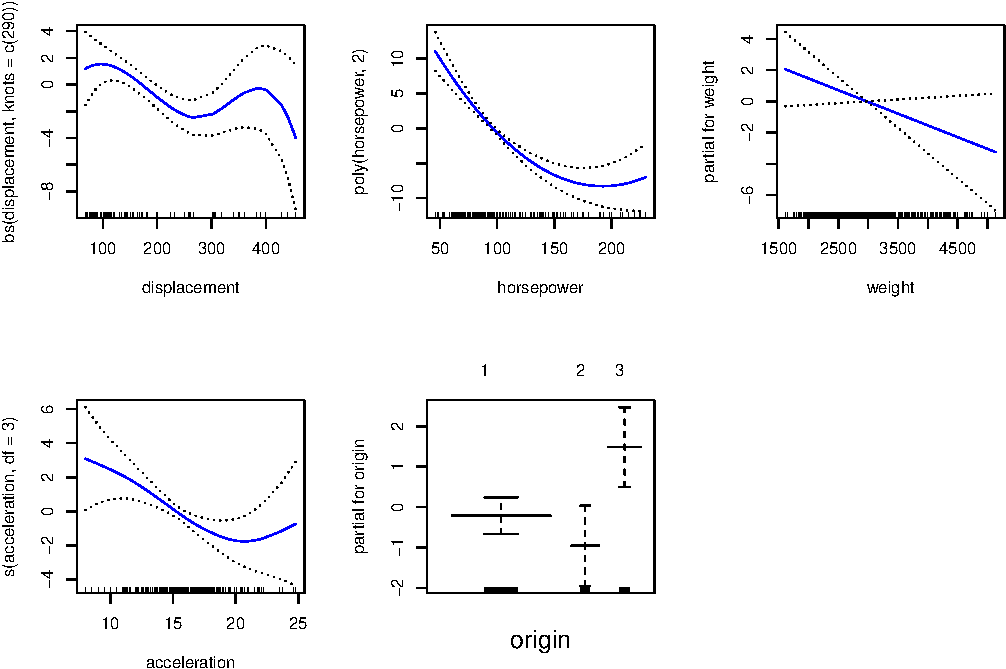
\includegraphics{RecEx7-sol_files/figure-latex/unnamed-chunk-7-1.pdf}

We see \texttt{displacement} has two peaks, \texttt{horsepower} has the
smallest CI for low values, the linear function in \texttt{weight} is
very variable for small and high values, \texttt{acceleration} looks
rather like a cubic function and there is a clear effect of
\texttt{origin}.

\end{document}
